\begin{figure}[t]
\centering
  \subfigure[$\gls{G}^{\prime} = \left(\gls{Neighbor}_{\gls{v}}, \gls{E}^{\prime}\right)$]{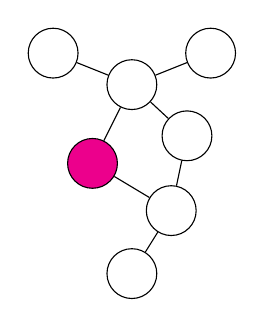
\begin{tikzpicture}
  \tikzstyle{node}=[circle,draw, minimum width=18pt, inner sep=0pt, fill=white]
  \tikzstyle{root}=[fill=magenta]

  \node[node, root] (1) at (0,    0)    {};
  \node[node]       (2) at (0.5,  1)    {};
  \node[node]       (3) at (1,    -0.6) {};
  \node[node]       (4) at (1.2,  0.35) {};
  \node[node]       (5) at (1.5,  1.4)  {};
  \node[node]       (6) at (-0.5, 1.4)  {};
  \node[node]       (7) at (0.5,  -1.4) {};

  \path (1) edge (2);
  \path (1) edge (3);
  \path (2) edge (4);
  \path (2) edge (5);
  \path (2) edge (6);
  \path (3) edge (4);
  \path (3) edge (7);
\end{tikzpicture}
}
\hspace{1cm}
  \subfigure[Distanz]{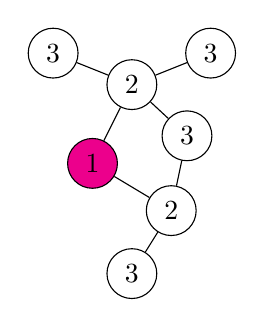
\begin{tikzpicture}
  \tikzstyle{node}=[circle,draw, minimum width=18pt, inner sep=0pt, fill=white]
  \tikzstyle{root}=[fill=magenta]

  \node[node, root] (1) at (0,    0)    {$1$};
  \node[node]       (2) at (0.5,  1)    {$2$};
  \node[node]       (3) at (1,    -0.6) {$2$};
  \node[node]       (4) at (1.2,  0.35) {$3$};
  \node[node]       (5) at (1.5,  1.4)  {$3$};
  \node[node]       (6) at (-0.5, 1.4)  {$3$};
  \node[node]       (7) at (0.5,  -1.4) {$3$};

  \path (1) edge (2);
  \path (1) edge (3);
  \path (2) edge (4);
  \path (2) edge (5);
  \path (2) edge (6);
  \path (3) edge (4);
  \path (3) edge (7);
\end{tikzpicture}
}
\hspace{1cm}
  \subfigure[Zentralität]{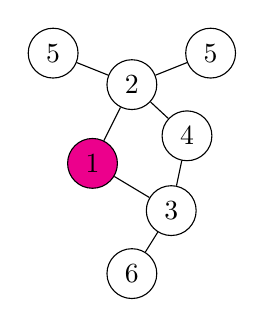
\begin{tikzpicture}
  \tikzstyle{node}=[circle,draw, minimum width=18pt, inner sep=0pt, fill=white]
  \tikzstyle{root}=[fill=magenta]

  \node[node, root] (1) at (0,    0)    {$1$};
  \node[node]       (2) at (0.5,  1)    {$2$};
  \node[node]       (3) at (1,    -0.6) {$3$};
  \node[node]       (4) at (1.2,  0.35) {$4$};
  \node[node]       (5) at (1.5,  1.4)  {$5$};
  \node[node]       (6) at (-0.5, 1.4)  {$5$};
  \node[node]       (7) at (0.5,  -1.4) {$6$};

  \path (1) edge (2);
  \path (1) edge (3);
  \path (2) edge (4);
  \path (2) edge (5);
  \path (2) edge (6);
  \path (3) edge (4);
  \path (3) edge (7);
\end{tikzpicture}
}
\hspace{0.6cm}
  \subfigure[Kanonisierung]{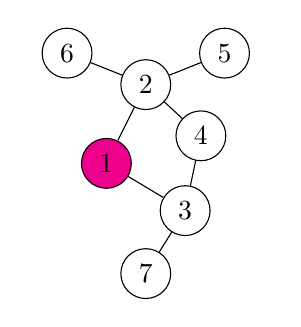
\begin{tikzpicture}
  \fill [white] (-1, 0) rectangle (2, 1) node {};  % Zentriere Graph.
  \tikzstyle{node}=[circle,draw, minimum width=18pt, inner sep=0pt, fill=white]
  \tikzstyle{root}=[fill=magenta]

  \node[node, root] (1) at (0,    0)    {$1$};
  \node[node]       (2) at (0.5,  1)    {$2$};
  \node[node]       (3) at (1,    -0.6) {$3$};
  \node[node]       (4) at (1.2,  0.35) {$4$};
  \node[node]       (5) at (1.5,  1.4)  {$5$};
  \node[node]       (6) at (-0.5, 1.4)  {$6$};
  \node[node]       (7) at (0.5,  -1.4) {$7$};

  \path (1) edge (2);
  \path (1) edge (3);
  \path (2) edge (4);
  \path (2) edge (5);
  \path (2) edge (6);
  \path (3) edge (4);
  \path (3) edge (7);
\end{tikzpicture}
}
\caption[Normalisierung]{Illustration der Normalisierung einer Nachbarschaft eines Knotens (rot) mit $7$ Knoten (a) zur Bestimmung einer eindeutigen Anordnung dieser.
Dazu werden die Nachbarschaftsknoten zuerst auf Basis ihrer Distanz zum Wurzelknoten gruppiert (b).
Innerhalb einer Gruppierung werden die Knoten auf Basis einer gegebenen Zentralitätsmetrik sortiert (c).
Im Anschluss werden Äquivalenzen in der Zentralität innerhalb einer Gruppe über eine Kanonisierung aufgelöst (d).
Gegebenenfalls muss die gefundene Ordnung danach auf die gewünschte Größe der Nachbarschaft zugeschnitten oder um Fakeknoten erweitert werden.}
\label{fig:raeumliche_faltung}
\end{figure}
